\documentclass[letterpaper, 10 pt, conference]{ieeeconf}

\IEEEoverridecommandlockouts

\overrideIEEEmargins

\makeatletter
\let\NAT@parse\undefined
\makeatother

\usepackage[dvipsnames]{xcolor}

\newcommand*\linkcolours{ForestGreen}

\usepackage{biblatex}
\usepackage{mathrsfs}
\usepackage{enumerate}
\usepackage{times}
\usepackage{graphicx}
\usepackage{amssymb}
\usepackage{gensymb}
\usepackage{amsmath}
\usepackage{breakurl}
\def\UrlBreaks{\do\/\do-}
\usepackage{url,hyperref}
\hypersetup{
colorlinks,
linkcolor=\linkcolours,
citecolor=\linkcolours,
filecolor=\linkcolours,
urlcolor=\linkcolours}

\usepackage{algorithm}
\usepackage{algorithmic}

\usepackage[labelfont={bf},font=small]{caption}
\usepackage[none]{hyphenat}

\usepackage{mathtools, cuted}

\usepackage[noadjust, nobreak]{cite}
\def\citepunct{,\,} % Style file defaults to listing references separately

\usepackage{tabularx}
\usepackage{amsmath}

\usepackage{float}

\usepackage{pifont}% http://ctan.org/pkg/pifont
\newcommand{\cmark}{\ding{51}}%
\newcommand{\xmark}{\ding{55}}%

\newcommand*\diff{\mathop{}\!\mathrm{d}}
\newcommand*\Diff[1]{\mathop{}\!\mathrm{d^#1}}
\newcommand*\imgres{600}

\newcommand*\GitHubLoc{https://github.com/Jeffrey-Ede/ALRC}

\newcolumntype{Y}{>{\centering\arraybackslash}X}

\usepackage[]{placeins}

\newcommand\extraspace{3pt}

\usepackage{placeins}

\usepackage{tikz}
\newcommand*\circled[1]{\tikz[baseline=(char.base)]{
            \node[shape=circle,draw,inner sep=0.8pt] (char) {#1};}}
            
\usepackage[framemethod=tikz]{mdframed}

\usepackage{afterpage}

\usepackage{stfloats}

\usepackage{atbegshi}
\newcommand{\handlethispage}{}
\newcommand{\discardpagesfromhere}{\let\handlethispage\AtBeginShipoutDiscard}
\newcommand{\keeppagesfromhere}{\let\handlethispage\relax}
\AtBeginShipout{\handlethispage}

\usepackage{comment}

\title{
CMPT 409: An Introduction to Quantum Computing \\
\large Assignment 2:  Part I (5-Page Report)
}

\author{Eric Sund | 301284359}

\begin{document}

\maketitle
\thispagestyle{empty}
\pagestyle{empty}


%%%%%%%%%%%%%%%%%%%%%%%%%%%%%%%%%%%%%%%%%%%%%%%%%%%%%%%%%%%%%%%%%%%%%%%%%%%%%%%%
\begin{abstract}

This paper serves as an introduction to the basics of our progress in Quantum Computing.  We first outline important prerequisite concepts.  This begins by observing how particles exhibit behaviors of waves, as a motivating factor to study Quantum Mechanics.  We build a foundation in this field of Physics by understanding its probabilistic nature in complex vector spaces (Hilbert Spaces).  We will see consequences of measurement collapsing the wave function, which acts as a complex-valued probability distribution.  Next, we see how Hilbert Spaces are ideal for modelling quantum bits, and how they can be represented with the Bloch Sphere.  Finally, we touch on the relevance, implications, and progress in quantum computing.

\end{abstract}

%%%%%%%%%%%%%%%%%%%%%%%%%%%%%%%%%%%%%%%%%%%%%%%%%%%%%%%%%%%%%%%%%%%%%%%%%%%%%%%%
\section{The Nature of Particles: Waves and Superposition}

Our current understanding of Classical Physics serves as a baseline for our progress in Classical Computing over the last 40 years.  Principles such as Moore's Law and algorithmic optimization show computational progress is not limited by our imagination, but rather what is physically possible.

Let us begin by considering particles and waves.  Particles are aggregations of sufficiently many atoms or molecules that can be assigned macroscopic properties such as volume, density, pressure, and temperature. \footnote{American Meteorology Society: http://glossary.ametsoc.org/wiki/Particle}  It came as a surprise to discover particles exhibit wave-like behavior when measured in the famous \textbf{Double Slit Experiment}, shown below.

\begin{figure}[h!]
  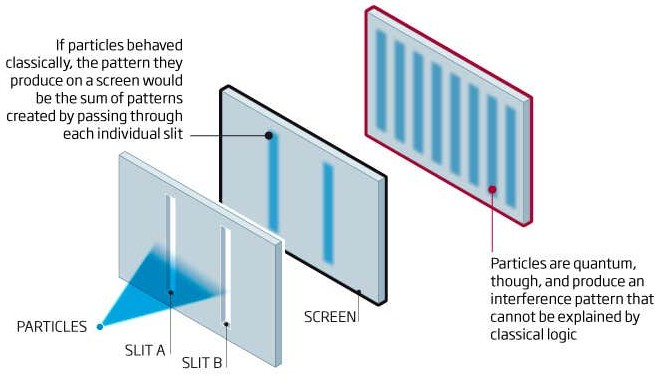
\includegraphics[width=\linewidth]{1.jpg}
  \caption{Photon particles exhibit wave-like behavior by producing interference patterns.  They do not pass straight through the slits.}
\end{figure}

This experiment helps us understand that particles behave like waves.  We see a discrete distribution of particles because constructive and destructive interference occurs when summing the waves exiting both slits.  That is, two waves can combine their amplitudes, creating larger or smaller waves.

Another famous experiment, \textbf{Schrödinger's Cat}, helps us understand the concept of \textbf{Superposition}.  That is, a quantum physical state can be represented as a linear combination of other possible states.  In Schrödinger's theoretical experiment, we place his cat, poison, a radioactive element and a Geiger counter in a box.  If the Geiger counter detects radioactivity, the poison container is broken which kills his cat.  The act of observation inside the box collapses the superposition of Schrödinger's Cat into one state.  Therefore, a possibly is:

\[ Cat = 0(Dead) + 1(Alive) \]

Revisiting the Double Slit Experiment, suppose \( \psi_1(x) \in \mathbb{C} \) and \( \psi_2(x) \in \mathbb{C} \) are complex amplitudes of a photon passing through numbered slits that touches a point, \(x\).  The probability the photon is present at \(x\) is \( P_1(x) = |\psi_1|^2 \) and \( P_2(x) = |\psi_2|^2 \).  Thus, when both slits are open, the probability of observing the photon would be the sum of both wave functions: \( P(x) = |\psi_1|^2 + |\psi_2|^2 \).  Consequently, the square of the absolute value of the complex amplitudes must indeed sum to 1.

Suppose instead of using functions representing continuous positions, we say the particle may be present in discrete positions.  All possible positions, \(|\Psi\rangle\) may be described as a linear combination of three other positions: \( |\Psi\rangle = \alpha|x_1\rangle + \beta|x_2\rangle + \gamma|x_3\rangle \) such that \(|\alpha|^2 + |\beta|^2 + |\gamma|^2 = 1\).  Recall our work over \( \mathbb{C} \), which requires multiplication by the complex conjugate.  \textit{Geometrically: reflection of complex number over the real horizontal axis.}  This gives ride to the \textbf{Born Rule}, which says the square of the absolute value of an amplitude is the probability of that state after measurement, and the sum of the squares of absolute values of all amplitudes is 1.

\section{Quantum States and Observables}

We've seen how wave functions represent positions of particles, and how particles can be in a superposition.  Intuitively, the states of a quantum physical system exist in complex vector spaces.  The quantum state is expressed using the \textbf{wave function}, a complex-valued probability distribution in a Hilbert Space.

For example, notice we can write the state as a linear combination of vectors.

\[
|\Psi\rangle = 
c_0 \begin{bmatrix}1 \\ 0 \\ \vdots \\ 0\end{bmatrix} + 
c_1 \begin{bmatrix}0 \\ 1 \\ \vdots \\ 0\end{bmatrix} + ... +
c_n \begin{bmatrix}0 \\ 0 \\ \vdots \\ 1\end{bmatrix}
\]

where \( |\Psi\rangle \) is the arbitrary state of the system, \(c_i\) is a complex weight (where \(|c_i|^2\) is the probability of a particle being at position \(i\), and the vector's components denote a particle's presence at some discrete position.  These vectors must form an orthonormal basis for this vector space.  We denote this vector space \( |\Psi\rangle \). \\

\textbf{Definition 2.1} We say \( |\Psi\rangle \) is a \textbf{ket}.  This is a generic vector whose complex entries denote the state of a quantum system.  Consequently, we say \( \langle\Psi| \) is a \textbf{bra}.  This is a complex conjugate transpose of a generic vector for a corresponding ket.

We now derive the following postulates from this definition:

\begin{enumerate}[I]
  \item Bra-kets \( \langle\psi|\phi\rangle \), are complex inner product, (generalized dot product), yielding a vector.
  \item Ket-bras \( |\phi\rangle\langle\psi| \), are outer product yielding a matrix.
  \item \( 1 = \langle\psi|\phi\rangle \)
\end{enumerate}

We've seen how a quantum state can be described by a ket, using one vector when the linear combination is simplified. \\

\textbf{Definition 2.2} When a state is described by one vector,
\[
|\psi\rangle = \alpha|0\rangle + \beta|1\rangle = 
\begin{bmatrix} \alpha \\ \beta \end{bmatrix}
\]

we say \( |\psi\rangle \) is a \textbf{pure state}.  Otherwise, it is a \textbf{mixed state}.  It is important to note that a mixed state is not the same as quantum superposition.  A mixed state's probabilities are classical (ie. non-negative and sum to one) whereas a pure state's are probability amplitudes. \\

Consider the pure state \( |\psi\rangle = \frac{|\psi_1\rangle + |\psi_2\rangle}{\sqrt{2}} \).  The coefficients \( \frac{1}{\sqrt{2}} \) are probability amplitudes.  To represent the probability of a mixed state \( |\phi\rangle = \frac{|\phi_1\rangle}{2} + \frac{|\phi_2\rangle}{2} \) being in \( |\phi_1\rangle \) or \( |\phi_2\rangle \) we may use a Density Matrix. \\

\textbf{Definition 2.3} A \textbf{Density Matrix}, or Density Operator, is a matrix representing the classical probability of a quantum mixed state being in a particular state.

\begin{equation}
p = \sum_{i} p_{i} |\psi_j\rangle \langle\psi_j|
\end{equation}

is the probability \( p_i \) the quantum system is in pure state \( |\psi_i\rangle \).

\section{Vector Spaces: Ideal Quantum Tools}

We can now show how states are represented nicely using complex vector spaces. \\

\textbf{Definition 3.1} Consider a physical space, perhaps with \(m\) discrete states, \( |\Phi\rangle \).  We can describe a larger space using the \textbf{outer product}, or \textbf{tensor product} as follows:

\begin{equation}
\begin{multlined}
|\Psi\rangle \otimes |\Phi\rangle = |\Psi\rangle \langle\Phi| =
\begin{bmatrix}\psi_0 \\ \psi_1 \\ \vdots \\ \psi_n \end{bmatrix}
\begin{bmatrix}\phi_0^* & \phi_1^* & \hdots & \phi_m^* \end{bmatrix} = \\
\begin{pmatrix}
\psi_1 \cdot \phi_1^* & \psi_1 \cdot \phi_2^* & \cdots & \psi_1 \cdot \phi_m^* \\
\psi_2 \cdot \phi_1^* & \psi_2 \cdot \phi_2^* & \cdots & \psi_2 \cdot \phi_m^* \\
\vdots  & \vdots  & \ddots & \vdots \\
\psi_n \cdot \phi_1^* & \psi_n \cdot \phi_2^* & \cdots & \psi_n \cdot \phi_m^*
\end{pmatrix}
\end{multlined}
\end{equation}

where \( \psi_i^* \) is the complex conjugate of \( \psi_i \) - we represent this by transposing a vector.  Note that we've combined a \( 1 \times n \) and \( 1 \times m \) space into an \( n \times m \) dimensional space.  Since we have that \( \mathbb{C}^n \otimes \mathbb{C}^m \) is isomorphic to \(  \mathbb{C}^{nm} \), we can rearrange our resulting matrix above into a vector.  That is:

\begin{equation}
|\Psi\rangle \otimes |\Phi\rangle =
\begin{bmatrix}\psi_0 \\ \psi_1 \\ \vdots \\ \psi_n \end{bmatrix} \otimes
\begin{bmatrix}\psi_0 \\ \phi_1 \\ \vdots \\ \phi_m \end{bmatrix} = 
\begin{bmatrix}\psi_0 \cdot \phi_0 \\ \psi_0 \cdot \phi_1 \\ \vdots \\ \psi_0 \cdot \phi_m \\
\psi_1 \cdot \phi_0 \\ \vdots \\ \psi_{n-1} \cdot \phi_m \\ \psi_{m} \cdot \phi_0 \\
\vdots \\ \psi_n \cdot \phi_m
\end{bmatrix}
\end{equation}

where the resulting column vector is isomorphic to the matrix from (1).

\textbf{Corollary} An \( n \times m \) tensor product is isomorphic to an \( nm \times 1 \) tensor product.  In vector form, we may interpret it as a vector in the larger \( \mathbb{C}^{nm} \) vector space.  Therefore, we can represent it as a linear combination of \( nm \) basis vectors.  That is, we have \( \mathbb{C}^{nm} = \) \textit{span} \{\( {|\psi_i\rangle \otimes |\phi_j\rangle } \)\} such that \( |\psi\rangle \) and \( |\phi\rangle \) are basis vectors for their corresponding vector spaces, for \( 1 \leq i \leq n \) and \( 1 \leq j \leq m \).

\textbf{Corollary} For some outer product \( tr(|\Psi\rangle \langle\Phi|) = |\Psi\rangle |\Phi\rangle \).  That is, the trace of the outer product is the \textbf{inner product}, where the inner product is the generalized dot product.\\

We've seen how arbitrary states in \( \mathbb{C}^{nm} \) can be represented as \( {|\psi\rangle \otimes |\phi\rangle } \) which we refer to as \textbf{separable states}.  Consider picking complex weights to write a general state in the larger space, say \( |\pi\rangle_{\Psi\Phi} \), as a linear combination of the basis vectors from the two smaller spaces.

\[
|\pi\rangle_{\Psi\Phi} = 
\sum_{i, j} c_{ij} |i\rangle_{\Psi} \otimes |j\rangle_{\Phi}
\]

for some basis \( |i\rangle \) in \( \Psi \) and some basis \( |j\rangle \) in \( \Phi \).  We're able to express \( |\pi\rangle \) because we have two complex weights from both spaces such that \( c_i \cdot c_j = c_{ij} \).  This produces \\

\[
|\Psi\rangle = \sum_{i} c_i |i\rangle,
|\Phi\rangle = \sum_{j} c_j |j\rangle
\]

\textbf{Definition 3.2} If for any \( c_i \), \( c_j \) we have \( c_i \cdot c_j \neq c_{ij} \) then the state \( |\pi\rangle \) is inseparable, thus \textbf{entangled}.  The most basic entangled states are \textbf{Bell States}, and they are:

\[
\frac{1}{\sqrt2}(|0\rangle_{\Psi} \otimes |0\rangle_{\Phi}) - |1\rangle_{\Psi} \otimes |1\rangle_{\Phi})
\]
\[
\frac{1}{\sqrt2}(|0\rangle_{\Psi} \otimes |0\rangle_{\Phi}) - |1\rangle_{\Psi} \otimes |1\rangle_{\Phi})
\]
\[
\frac{1}{\sqrt2}(|0\rangle_{\Psi} \otimes |1\rangle_{\Phi}) - |1\rangle_{\Psi} \otimes |0\rangle_{\Phi})
\]
\[
\frac{1}{\sqrt2}(|0\rangle_{\Psi} \otimes |1\rangle_{\Phi}) - |1\rangle_{\Psi} \otimes |0\rangle_{\Phi})
\]

where \( |0\rangle \) = \( \begin{bmatrix} 1 \\ 0 \end{bmatrix} \) and \( |1\rangle \) = \( \begin{bmatrix} 0 \\ 1 \end{bmatrix} \), the \textbf{computational basis}.
\\

Recall our claim that quantum Physics is probabilistic in nature.  That is, a measurement will collapse a superpostion into a particular state.  We've seen how taking the square of an absolute value of a probability amplitude returns the classical probability of being in that state.  The Expected Value (average value) is the average value of measurement.

For example, the probability \( |\psi\rangle = \alpha|0\rangle + \beta|1\rangle \) is in state \( |0\rangle \) is \( |\alpha|^2 \), and \( |\beta|^2 \) it is in \( |1\rangle \).  The average value would be \( |\alpha|^2 - |\beta|^2 \). \\

Let

\[
Z = |0\rangle\langle0| - |1\rangle\langle1|
\]
\[
=
\begin{bmatrix} 1 \\ 0 \end{bmatrix}
\begin{bmatrix} 1 & 0 \end{bmatrix} -
\begin{bmatrix} 0 \\ 1 \end{bmatrix}
\begin{bmatrix} 0 & 1 \end{bmatrix}
\]
\[
=
\begin{bmatrix}
1 & 0 \\
0 & 0
\end{bmatrix} -
\begin{bmatrix}
0 & 0 \\
0 & 1
\end{bmatrix} =
\begin{bmatrix}
1 & 0 \\
0 & -1
\end{bmatrix}
\]

be the observable operator of the system.\\

The expected value of the system is expressed in terms of the \textit{Z} \textbf{linear operator} as follows:

\begin{equation}
\langle\psi|Z|\psi\rangle = \langle\psi|0\rangle \langle0|\psi\rangle - \langle\psi|1\rangle \langle1|\psi\rangle = |\alpha|^2 - |\beta|^2,
\end{equation}

or simply \( \langle Z \rangle \).  An operator acting on a state is like a matrix product.  Although this example used the computational basis, we may use any basis to compute an expected value.  As a consequence, Hermitian operators are diagonalizable - you can find a basis (coordinate system) comprised entirely of eigenvectors.  Tracking evolution of the observable simply means remembering coefficients of these eigenvectors.  This doesn't work for \( \mathbb{R} \) and is probably the biggest reason to work over \( \mathbb{C} \). \\

To this point, we've seen how the classical probability of a quantum system being in a particular state is the square of the absolute value of that probability amplitude.  We denote this as the \( L^2 \) norm, or Euclidean Norm, and define additional norms:

\textbf{Definition 3.3} Given a vector
\[
|\Psi\rangle =
\begin{bmatrix} \psi_0 \\ \vdots \\ \psi_n \end{bmatrix}
\]

such that \( |\Psi\rangle \in \mathbb{C}^n \), the \( L^1 \) norm is defined by

\[
|\Psi|_1 = \sum_{i = 0}^n |\psi_i|,
\]

the \( L^2 \) norm is defined by

\[
|\Psi| = \sum_{i = 0}^n |\psi_i|^2,
\]

and more generally, the \( L^p \) norm is defined by

\[
||\Psi||_p = 
\sqrt[\leftroot{-2}\uproot{2}p]{ \sum_{i = 0}^n \psi_i^p }.
\]

\section{The Bloch Sphere}

Consider a \textbf{quantum bit}, that is, some vector in 2-dimensional Hilbert Space.  We say a \textbf{qbit} is in superposition, meaning it can have arbitrary values in its two components until it is measured, collapsing it into a particular state.  Quantum bits are in a superposition of two states, whereas classical bits can be in either 0 or 1 exclusively.

The \textbf{Bloch sphere} is a convenient geometric representation of a qbit's pure state.

Suppose we have some qbit \( |\Psi\rangle \in \mathbb{C}^2 \).  By the Born Rule:

\[ |\Psi\rangle =
\begin{bmatrix} \alpha \\ \beta \end{bmatrix};  \alpha, \beta \in \mathbb{C};  |\alpha|^2 + |\beta|^2 = 1.
\]

Using the trigonometric identity \( sin^2(\theta) + cos^2(\theta) = 1 \), we may write \( \alpha = cos(\theta) \) and \( \beta = sin(\theta) \) for \( \theta \in \mathbb{R} \) which yields

\[
|\Psi\rangle = \begin{bmatrix} cos(\theta) \\ sin(\theta) \end{bmatrix}.
\]  Since we're working in a complex vector space, we may use Euler's Formula to further represent the qbit in a position around another circle (another dimension).  Note, \textbf{Euler's Formula} is \( e^{i\pi} = -1 \).  We may introduce some scaling factor, say \( \phi \) to rotate our desired position around the complex circle, \( e^{\phi \cdot i} \) This is a convenient way of representing a qbit in 3 dimensions on a sphere.  Therefore, we can represent our qbit as

\[
|\Psi\rangle =
\begin{bmatrix} cos(\theta) \\ e^{\phi \cdot i} sin(\theta) \end{bmatrix},
\]

and in dirac notation,

\[
|\Psi\rangle = cos(\frac{\theta}{2}) |0\rangle + e^{\phi \cdot i} sin(\frac{\theta}{2}) |1\rangle
\]

such that \( 0 \leq \theta \leq \pi \) and \( 0 \leq \phi < 2\pi \).

We see that \( |0\rangle \) is the north pole because we take \( \theta = 0 \) and \( |1\rangle \) is the south pole because we take \( \theta = \pi \).

\begin{figure}[h!]
    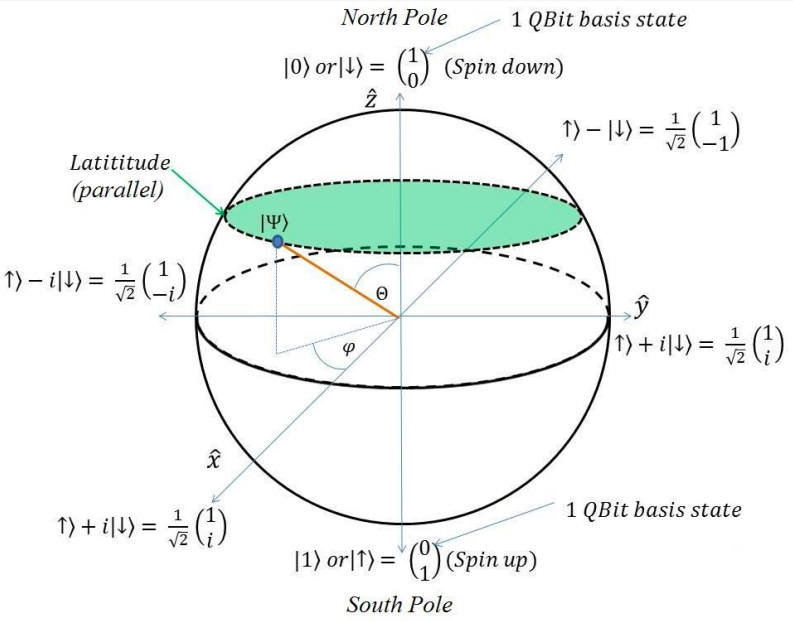
\includegraphics[width=\linewidth]{sphere.png}
    \caption{Pure states are represented on the surface of a sphere, (mixed states inside) by taking unitary transformations resulting in vectors.  This lets us find amplitudes and measure qbits.}
\end{figure}

\section{Quantum Computation}

Now we see how computations can be performed with Quantum Physics.  We use concepts from Linear Algebra to mirror concepts in quantum computing.  We derive the following postulates:

\begin{itemize}
   \item Qbits are represented in in 2-D complex Hilbert Spaces.  Let this be \( \mathscr{H} \).  We have that \( \mathscr{H} =  span_\mathbb{C} \{ {|0\rangle, |1\rangle } \)\}.
   \begin{itemize}
     \item The state of a qbit is represented by a vector in \( \mathscr{H} \).
   \end{itemize}
   \item For qbits with more than 2 dimensions, say n, we may tensor a qbit with itself n times.
   \begin{itemize}
     \item \( \mathscr{H}^{\otimes n} \)
   \end{itemize}
   \item The entire state in space may be described by vectors with \( L^2 \) norm of 1.  These are vectors (qbits) on the Bloch Sphere.
   \begin{itemize}
     \item Let this be the set: \( \{v \in \mathscr{H} \) such that \( \langle v|v\rangle = 1\} \)
   \end{itemize}
   \item The computational basis are othonormal.  That is, they are orthogonal (perpendicular; inner product of 0) and have an \( L^2 \) norm 1.
   \begin{itemize}
     \item \( |0\rangle = \begin{bmatrix} 1 \\ 0 \end{bmatrix} \) and \( |1\rangle = \begin{bmatrix} 0 \\ 1 \end{bmatrix} \)
   \end{itemize}
   \item When qbits are in superposition, they are represented as a linear combination of the orthonormal basis vectors with \( L^2 \) norm of 1 on the Bloch Sphere.
   \begin{itemize}
     \item For example using the computational basis, we can say: \( \frac{1}{\sqrt{2}}|0\rangle + \frac{1}{\sqrt{2}}|1\rangle \).\\
   \end{itemize}
\end{itemize}

Arguably, the most important concept from Linear Algebra is what defines Quantum Logic Gates.  We assume the reader is familiar with Classical Logic Gates, such as AND, OR, NOT gates, for example.  In the quantum world, these are \textbf{Unitary Operators}.  That is, they are square matrices (almost always \( 2 \times 2\)) with complex components.  We use these to act on the state space by taking the product of such matrix with a vector.  They do preserve the norm of the vectors and transform vectors into new states.  Consequently, we can build quantum logic circuits with Unitary Operators!  Below are some example operators.\\

The identity function, \( f(x) = x \):
\[
|0\rangle \to |0\rangle \quad \quad |1\rangle \to |1\rangle,
\]
\[
\begin{bmatrix}
1 & 0 \\
0 & 1
\end{bmatrix}
\begin{bmatrix} 1 \\ 0 \end{bmatrix} =
\begin{bmatrix} 1 \\ 0 \end{bmatrix}
\quad \quad
\begin{bmatrix}
1 & 0 \\
0 & 1
\end{bmatrix}
\begin{bmatrix} 0 \\ 1 \end{bmatrix} =
\begin{bmatrix} 0 \\ 1 \end{bmatrix}
\]

The negation function, \( f(x) = \neg x \):
\[
|0\rangle \to |1\rangle \quad \quad |1\rangle \to |0\rangle,
\]
\[
\begin{bmatrix}
0 & 1 \\
1 & 0
\end{bmatrix}
\begin{bmatrix} 1 \\ 0 \end{bmatrix} =
\begin{bmatrix} 0 \\ 1 \end{bmatrix}
\quad \quad
\begin{bmatrix}
0 & 1 \\
1 & 0
\end{bmatrix}
\begin{bmatrix} 0 \\ 1 \end{bmatrix} =
\begin{bmatrix} 1 \\ 0 \end{bmatrix}
\]

The constant zero function, \( f(x) = 0 \):
\[
|0\rangle \to |0\rangle \quad \quad |0\rangle \to |0\rangle,
\]
\[
\begin{bmatrix}
1 & 1 \\
0 & 0
\end{bmatrix}
\begin{bmatrix} 1 \\ 0 \end{bmatrix} =
\begin{bmatrix} 1 \\ 0 \end{bmatrix}
\quad \quad
\begin{bmatrix}
1 & 1 \\
0 & 0
\end{bmatrix}
\begin{bmatrix} 0 \\ 1 \end{bmatrix} =
\begin{bmatrix} 1 \\ 0 \end{bmatrix}
\]

The constant one function, \( f(x) = 1 \):
\[
|1\rangle \to |1\rangle \quad \quad |0\rangle \to |1\rangle,
\]
\[
\begin{bmatrix}
0 & 0 \\
1 & 1
\end{bmatrix}
\begin{bmatrix} 1 \\ 0 \end{bmatrix} =
\begin{bmatrix} 0 \\ 1 \end{bmatrix}
\quad \quad
\begin{bmatrix}
0 & 0 \\
1 & 1
\end{bmatrix}
\begin{bmatrix} 0 \\ 1 \end{bmatrix} =
\begin{bmatrix} 0 \\ 1 \end{bmatrix}
\]

It follows that \textbf{Measurement Operators} are Projection Operators, which are operations which result in a projection.  This transforms quantum bits into classical bits.  When resulting state is probabilistic, not deterministic, as we've seen through the Born Rule and the Expected Value in equation (4).

When we perform quantum computations, we are not limited to the computational basis.  We may use others, such as the Hadamard Basis for qbits:

\[
|+\rangle = \frac{|0\rangle + |1\rangle}{\sqrt{2}} =
\frac{1}{\sqrt{2}}\begin{bmatrix} 1 \\ 1 \end{bmatrix},
|-\rangle = \frac{|0\rangle - |1\rangle}{\sqrt{2}} =
\frac{1}{\sqrt{2}}\begin{bmatrix} 1 \\ -1 \end{bmatrix}.
\]

Note that \( |+\rangle \) and \( |-\rangle \) differ only by a \(-\) relative phase.  From Euler's Identity, we have that \( -1 = e^{i\pi} \).  We can think of this as rotating \( \pi \) radians around the complex circle, which implies interference.

\textbf{Definition 5.1} Interference is the concept of wave amplitudes cancelling, or adding to produce new wave amplitudes.  \textbf{Constructive interference} results in two wave amplitudes summing to produce a larger one.  \textbf{Destructive interference} results in two wave amplitudes summing to produce a smaller one, or potentially a \textit{zero amplitude}.\\

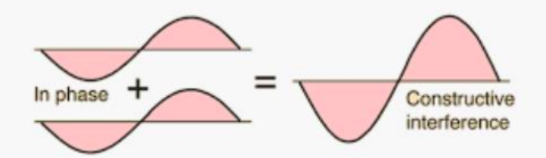
\includegraphics[width=230px]{phase1.png}
\hspace*{+0.35cm}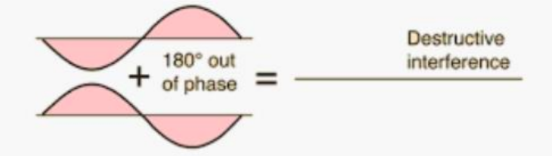
\includegraphics[width=230px]{phase2.png}\\

Suppose we use the Hadamard Basis and obtain a particular state in our physical system:

\[
\frac{|+\rangle + |-\rangle}{\sqrt{2}} =
\frac{|0\rangle + |1\rangle}{2} + 
\frac{|0\rangle - |1\rangle}{2} = |0\rangle.
\]
\[
\frac{|-\rangle + |+\rangle}{\sqrt{2}} =
\frac{|1\rangle + |0\rangle}{2} + 
\frac{|1\rangle - |0\rangle}{2} = -|1\rangle.
\]

What happened here?  In the first equation, the \( |1\rangle \) amplitudes interfered destructively by cancelling out, whereas \( |0\rangle \) amplitudes interfered constructively.  The exact opposite happens in the second equation.  Note the second equation results in a difference of \( - \) from \( |1\rangle \).  The difference in phase is not applied to one state in the super position, but the whole state.  We call this \textbf{global phase}.  We can visualize what is happening here by looking at a projection of the Bloch Sphere into \(\mathbb{C}^2\).

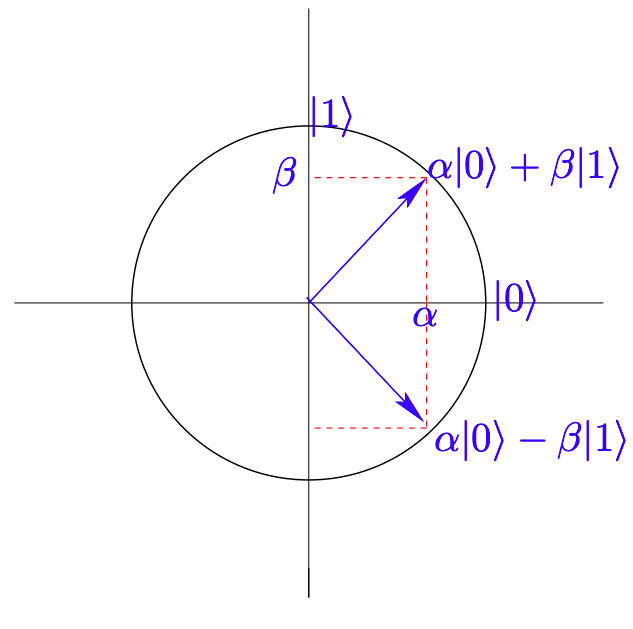
\includegraphics[width=230px]{circle.png}

With an understanding of interference, we can infer how decoherence, and interference may be challenges in quantum computation.  \textbf{Decoherence} is the challenge of keeping qbits undisturbed for long enough to have useful measurements.  Qbits have unwanted interaction with the surrounding environment giving rise to an irreversible process in which a pure state becomes a mixed state.

One of the main problems with quantum computation is the amount of resources required, due to qbits being in superposition.  In one computational step, a classical computer with a 64-bit architecture can process 64 bits.  Contrast this to a quantum computer with a 64-bit architecture, processing \( 2^{64} \) bits in one computational step.  Building hardware to support such a quantum computer is most certainly nontrivial.

In classical computing we require hundreds of bits to perform meaningful calculations.  We apply classical gates to classical bits to perform operations.  This is the same case in the quantum world, except we apply quantum gates to qubits, which corresponds to multiplying a vector and matrix in a \textbf{QPU (Quantum Processing Unit)}.

A quantum gate is a matrix, which is an procedure transforming preexisting probability amplitudes in the QPU.  However, quantum gates are not physical structures as classical gates are, which requires us to re-think how a quantum algorithm should run.  Classical algorithms may be run on a quantum computer, but quantum algorithms may only be run on quantum computers.  This is because they are inherently quantum, or use some essential feature of quantum computation such as superposition or entanglement.

Quantum Algorithms are more difficult to code, because they involve exploiting the underlying structure of a problem.  Quantum algorithms have proven to be effective in integer factorization, optimization, and graph isomorphism problems.  Notable examples include \textbf{Peter Shor's integer factorization algorithm}, and \textbf{Lov Grover's search algorithm}.

Algorithms that may be worth our time to code and run on a quantum computer should be those with super-polynomial speedups.  These are not seen in Grover’s algorithm, which only decreases its search running time from \(O(n)\) to \(O\sqrt{n}\).  These speedups do happen in graph isomorphism problems, cryptographic methods, NP problems, and quantum physical simulations.

\section{References}

\begin{itemize}
\item \textbf{Double Slit}\\ https://d1o50x50snmhul.cloudfront.net \\ /wp-content/uploads/2011/09/28285901.jpg\\

\item \textbf{Bloch Sphere}\\
https://arxiv.org/ftp/arxiv/papers/1512/1512.02942.pdf\\

\item \textbf{Bloch Sphere Projection}\\ https://www.cl.cam.ac.uk/teaching/0910/QuantComp/notes.pdf\\

\textit{Additional concepts are from Dr. Steven Pearce's CMPT 409 Power Point slides.}
\end{itemize}

\end{document}
